\documentclass[12pt]{scrartcl}
\usepackage[ngerman]{babel}


\usepackage{amsmath, amssymb}

\usepackage{ulem} % double underline

\usepackage{array}  % for the tables

\usepackage{nameref}  % for referencing with name

\usepackage{hyperref}  % for hyperlinks

\usepackage{mathrsfs}

\usepackage{graphicx}  % for the images

\usepackage{glossaries}

\usepackage{xcolor, colortbl}

\usepackage{lmodern}

\usepackage{tcolorbox}

\usepackage{pgfplots}

\usepackage{tabto}

\usepackage{setspace}

\pgfplotsset{compat=1.15}

\usetikzlibrary{arrows}

\definecolor{Gray}{gray}{0.85}

\setlength{\parindent}{0pt}

\definecolor{qqwwzz}{rgb}{0,0.4,0.6}
\definecolor{qqwuqq}{rgb}{0,0.39,0}

% hyperlinks
\hypersetup{
    colorlinks,
    citecolor=black,
    filecolor=black,
    linkcolor=black,
    urlcolor=black
}

% for coloring in text %

\newcommand{\red}[1]{\textcolor{red}{#1}}

\bibliographystyle{IEEetran}




\author{David Jäggli}

\title{Analysis Integralrechnung}



% ---------- Begin Main Document ----------- %



\begin{document}

\maketitle

\tableofcontents

\newpage
\section{Das unbestimmte Integral}
Bei der Integralrechnung haben wir die umgekehrte Aufgabenstellung als bei der Differenzialrechnung.
Anstatt Ableitung (quasi Aufleitung).\\
Fragenstellung: welche Funktion $F'(x)$ gibt abgeleitet $f(x)$.\\
\textbf{Beispiel:}\\
\[f(x) = x^3+2x^2+5x-6 \]
\[F(x) = \frac{1}{4}x^4+\frac{2}{3}x^3+\frac{5}{2}x^2-6x+c\] \\
\[ \int \sqrt[5]{x^4} \, dx = \int x^{\frac{4}{5}} = \frac{x^{\frac{4}{5} + 1}}{\frac{4}{5} + 1} = \frac{x^{\frac{9}{5}}}{\frac{9}{5}} = \uuline{\frac{9}{5} \cdot x^{\frac{5}{9}}}\]
\\
Wobei: $F(x) = \int f(x) \,dx$ \\

\noindent
\textbf{Weiter zu beachten:}
\begin{itemize}
    \item Weil Konstante c fehlt, ist es ein unbestimmtes Integral.
    \item Nicht jede Funktion hat eine Stammfunktion.
\end{itemize}


\renewcommand{\arraystretch}{1.5}
\begin{tcolorbox}
    \textbf{Man bezeichnet:}\\
    \begin{tabular}{cl}
        $f(x)$            & als \textbf{Integrand} = Funktion die hinter/unter dem Integral steht\\
        $\int f(x) \, dx$ & als \textbf{unbestimmtes Integral} \\
        $F(x) + c$        & als \textbf{Stammfunktion} \\
        $x$               & die \textbf{Integrationsvariable} \\
        $c$               & als \textbf{Integrationskonstante} \\
    \end{tabular}
\end{tcolorbox}


\newpage
\subsection{Integrationsregeln}\label{Integrationsregeln unb. Integrale}
Bei allen Integrationen immer ganz am Schluss noch die Konstante $c$ hinschreiben.

\subsubsection{Potenz}
\[\int x^n \, dx = \frac{1}{n + 1}x^{n + 1}\]

\subsubsection{Faktoren}
Ein konstanter Faktor kann vor das Integrationszeichen genommen werden.
\[\int a \cdot f(x) \, dx = a \cdot \int f(x) \, dx\]


\subsubsection{Summe}
Das Integral aus einer Summe von Funktion ist gleich der Summe der Integrale
der einzelnen Funktionen.
\[\int f(x) + g(x) \, dx = \int f(x)\, dx + \int g(x) \, dx\]

\subsubsection{Multiplikation}
Ein Produkt von Funktionen kann nicht einfach voneinander getrennt werden wie bei der Summe\\
Das heisst:\\
\[\int f(x) \cdot g(x) \, dx \neq \int f(x) \, dx \cdot \int g(x) \, dx\]
\vspace*{20px}\\
\textbf{siehe stattdessen: \hyperref[sec:Partielle-Integration]{Kapitel \ref{sec:Partielle-Integration} Partielle Integration}}

\newpage
\subsection{Integration von weiteren elementaren Funktionen}
Exponentielle Funktionen:
\begin{center}
    \renewcommand{\arraystretch}{2}
    \begin{tabular}{| m{5em} | m{25em} | }
        \hline
        $E_1$ & $\int e^x \, dx = e^x + c$ \\
        \hline
        $E_2$ & $\int e^{ax + b} \, dx = \frac{1}{a} \cdot e^{ax+b} + c$ \\
        \hline
        $E_3$ & $\int a^x \, dx = \frac{a^x}{ln(a)} + c$ \qquad \qquad \quad für $a \in \mathbb{R}_{+}^{*}$ und $a \neq 1$\\
        \hline
    \end{tabular}
\end{center}
Logarithmische Funktionen:
\begin{center}
    \renewcommand{\arraystretch}{2}
    \begin{tabular}{| m{5em} | m{25em} | }
        \hline
        $L_1$ & $\int ln(x) \, dx = x \cdot ln(x) - x + c$ für $x \in \mathbb{R}_{+}^{*} $\\
        \hline
        $L_2$ & $\int ln(ax + b) \, dx = \frac{1}{a}[(ax + b) \cdot ln(ax+b) - (ax + b)] + c$ \\
        \hline
        $L_3$ & $\int log_ax \, dx = \frac{1}{ln(a)}(x \cdot ln(x) - x) + c$ für $x \in \mathbb{R}_{+}^{*}$ \\
        \hline
    \end{tabular}
\end{center}

\newpage

\section{Das bestimmte Integral}
\subsection{Die Berechnung des bestimmten Integrals}
Mithilfe der Integralrechnung kann man z.B. eine Fläche unter einer Kurve in einem 
gewissen Abschnitt berechnen. \\
\noindent
Es gilt: 

\[\int_{a}^{b} f(x) \, dx = F(b) - F(a)\]

Wobei F die Stammfunktion von f(x) ist.\\

\noindent
\textbf{Vorgehensweise für die Berechnung des bestimmten Integrals} 
\begin{itemize}
    \item Bestimmung der Stammfunktion $F(x)$
    \item Bilden der zwei eingesetzten Werte $F(a)$ und $F(b)$
    \item Subtraktion der von $F(b) - F(a)$ ergibt das gesuchte Integral.
\end{itemize}
Die Integrationskonstante c im bestimmten Integral fällt weg und muss somit nicht
berücksichtigt werden.


\subsection{Bestimmtes Integral und Flächeninhalt}
Das bestimmte Integral kann jedoch nicht uneingeschränkt mit dem Flächeninhalt gleichgesetzt 
werden. Geht die Ursprungsfunktion in den negativen y-Wertebereich
ergeben sich negative Flächen, was nicht sehr sinnvoll ist.\\
\noindent
Will man die gesamte Fläche zwischen der Funktionskurve und der x-Achse herausfinden, muss man
die einzelnen Flächen zwischen den Nullpunkten einzeln berechnen und den Absolutwert
davon nehmen.\\

\noindent
\textbf{Vorgehensweise für die Berechnung der Fläche}
\begin{enumerate}
    \item Berechnen der Nullstellen von $f(x)$.
    \item Die Integrale einzeln rechen.
    \item Die Beträge aller Resultate addieren.
\end{enumerate}

\newpage

\noindent
\textbf{Anschaungs-Beispiel:} \\
Bei folgendem Beispiel ist die Kurve $-x^2 + 6x$ gegeben. Die blaue Fläche würde man mit folgender Formel
berechnen:
\[{\int_{0}^{6}  -x^2 + 6x\,dx }\]
resp.
\[F(6) - F(0)\]
\begin{tikzpicture}[line cap=round,line join=round,>=triangle 45,x=1cm,y=1cm]
    \begin{axis}[
    x=1.5cm,y=0.75cm,
    axis lines=middle,
    ymajorgrids=true,
    xmajorgrids=true,
    xmin=-1,
    xmax=8,
    ymin=-2,
    ymax=10,
    xtick={-1,0,...,8},
    ytick={-2, 0,...,10},]
    \clip(-2.3866006234132833,-10.726450007228292) rectangle (8.78724606115888,24.428863974258505);
    \draw[line width=0.8pt,color=qqwwzz,fill=qqwwzz,fill opacity=0.1, smooth,samples=50,domain=0:6] plot(\x,{0-(\x)^(2)+6*(\x)}) -- (6,0) -- (0,0) -- cycle;
    \draw[line width=2pt,color=qqwuqq,smooth,samples=100,domain=-2.3866006234132833:8.78724606115888] plot(\x,{0-(\x)^(2)+6*(\x)});
    \begin{scriptsize}
    \draw[color=qqwuqq] (-1.4019600865874071,-10.015320730631826) node {$f$};
    \end{scriptsize}
    \end{axis}
\end{tikzpicture}


\newpage
\subsection{Integrationsregeln für bestimmte Integrale}
Für Faktor- und Additionsregel siehe auch Kapitel \ref{Integrationsregeln unb. Integrale}


\renewcommand{\arraystretch}{1.5}
\begin{center}
    \begin{tabular}{ | m{10em} m{26em} | }
        \hline
        Faktorregel: &  \[\int_a^b c \cdot f(x) dx = c \cdot \int_a^b f(x) dx\]\\ 
        \hline
        Additionsregel: & \[\int_a^b f(x) \pm g(x) dx = \int_a^b f(x) \pm \int_a^b g(x) dx\] \\ 
        \hline
        Vertauschungsregel: & \[\int_{\red{a}}^{\red{b}} f(x) dx = \red{-}\int_{\red{b}}^{\red{a}} f(x) dx\] \\ 
        \hline
        Zerlegungsregel \newline für $a < c < b$ gilt: & \[\int_a^b f(x) dx = \int_a^c f(x) dx + \int_c^b f(x)\] \\ 
        \hline
        Vergleichsregel \newline [Bedingung\footnotemark{}] & \[\int_a^b g(x) dx \leq \int_a^b f(x) dx\] \\ 
        \hline
        Fläche einer Linie: & \[\int_a^a f(x) dx = 0\] \\ 
        \hline
    \end{tabular}
\end{center}

\footnotetext{Wenn $f(x)$ und $g(x)$ im Intervall $a\leq x \leq b$ stetig sind und im Intervall gilt immer $f(x) < g(x)$}

\subsection{Integrationsvariable ungleich 'x'}
Die Integrationsvariable muss nicht immer x sein. Nach welcher Variabel integriert wird, 
wird am Schluss mit 'd' angegeben. Also $dx$ für $x$ oder $dy$ für $y$.

\newpage
\section{Substitutionsmethoden}
\subsection{Lineare Substitution}

\renewcommand{\arraystretch}{1.5}
\begin{center}
    \begin{tabular}{ | m{18em} | m{18em} | }
        \hline
        Zu berechnendes Integral: & $\int (ax + b)^n dx$ \\ 
        \hline
        Berechnung von z:  & $z = ax + b$ \\ 
        \hline
        Integral berechnen:  & $\frac{1}{a}\int z^n dz = \frac{1}{a \cdot (n+1)}z^{n+1}$ \\ 
        \hline
        Zurücksubstituieren: & $\frac{1}{a \cdot (n + 1)}(ax+b)^{n + 1} + c$ \\
        \hline
    \end{tabular}
\end{center}

Allgemeine finale Formel:
\[ \frac{1}{a \cdot (n + 1)}(ax+b)^{n + 1} + c\]


Formelsammlung für einzelne Fälle:
\renewcommand{\arraystretch}{1.5}
\begin{center}
    \begin{tabular}{ | m{18em} | m{18em} | }
        \hline
        \textbf{\underline{Fall}} & \textbf{\underline{Lösung}} \\ 
        \hline
        $\int (ax + b)^n \, dx$  & $\frac{1}{a \cdot (n+1)}(ax + b)^{n+1} + c$ \\ 
        \hline
        $\int \sqrt{ax + b} \,\,dx$  & $\frac{2}{3a}(ax + b)^{\frac{3}{2}} + c$ \\ 
        \hline
        $\int e^{ax + b} \, dx$ & $\frac{1}{a} \cdot e^{ax + b} + c$ \\
        \hline
    \end{tabular}
\end{center}



\subsubsection{Spezialfall: die logarithmische Integration}
Falls die Substitution z von der Form z = $\frac{1}{g(x)}$ ist, oder wenn der Integrand
die Form $\frac{g^(x)}{g(x)} dx$ hat, ergibt sich für die Lösung eine allgemeine Formel.

\[\int \frac{g'(x)}{g(x)} dx = ln|g(x)| + c\]

Funktioniert auch, wenn im Zähler ein Vielfaches von der Ableitung steht $\rightarrow$ Vielfaches 
aus der Integration herausnehmen.


\newpage
\section{Integrierbarkeit}
Im Gegensatz zu der Differenzialrechnung sind endliche Sprünge und Knicke kein Problem.
Nur bei Polen kann nicht integriert werden.

\subsection{Endlicher Sprung und Knick}
Folgende 2 Beispiele sind integrierbar. Dafür muss jeweils die Stammfunktion der
einzelnen Funktionen gebildet, Fläche berechnet und addiert werden.
\begin{center}
    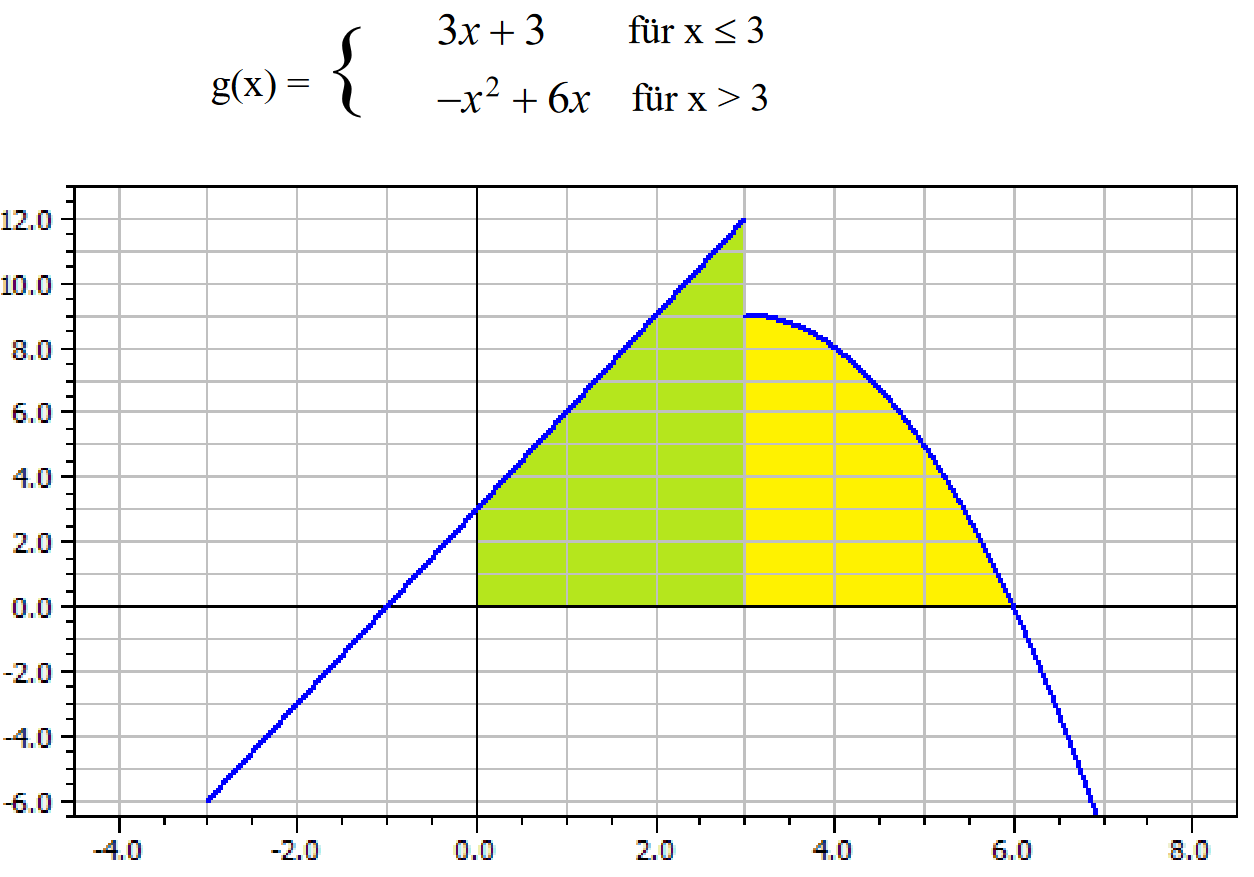
\includegraphics[width=12cm]{img/finite-jump.png}\\
    \vspace*{10px}
    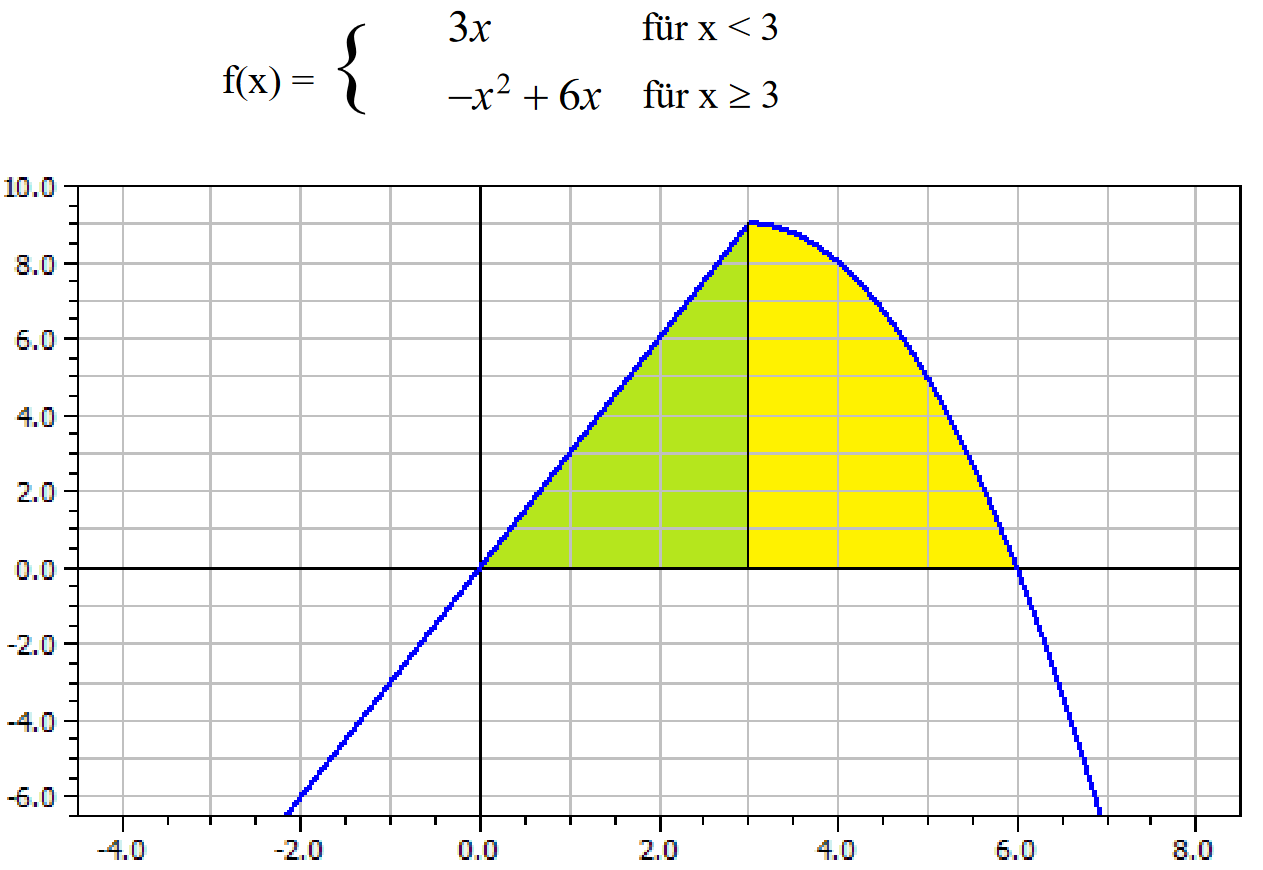
\includegraphics[width=12cm]{img/kink.png}
\end{center}


\newpage
\subsection{Pole}
Beide Funktionen, sowohl die Rote wie auch die Blaue, können nicht komplett integriert werden, 
da sie einen Pol (unendlicher Sprung in der y-Achse) haben. Vor und nach dem Pol sind die Funktionen
jedoch problemlos integrierbar.

\begin{center}
    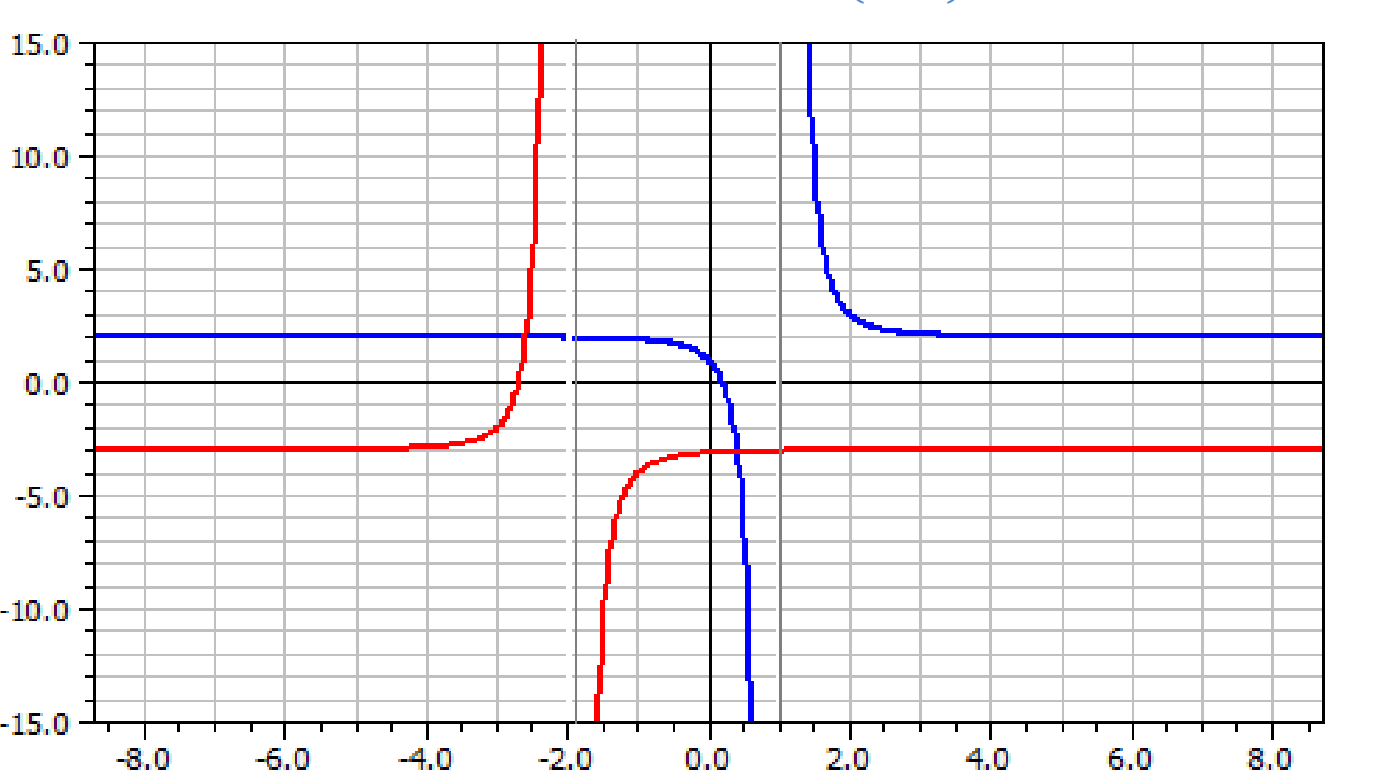
\includegraphics[width=13cm]{img/two-poles.png}
\end{center}

\newpage
\section{Partielle Integration} \label{sec:Partielle-Integration}
\subsection{Einleitung}
Die Produktregel der Diff. rechnung: \tab $(f(x) \cdot g(x))' = f'(x) \cdot g(x) + f(x) \cdot g'(x)$.
\vspace*{10px}

Umgeformt ergibt sich: \tab $f(x) \cdot g'(x) = (f(x) \cdot g(x))' - f'(x) \cdot g(x)$
\vspace*{10px}

Integriert \& vereinfacht: \tab $ \int f(x) \cdot g'(x) \, dx = f(x) \cdot g(x) - \int f'(x) \cdot g(x) \, dx $
\vspace*{25px}

\subsection{Anleitung mit Beispiel}
Ziel: Das Integral von $I = \int x \cdot 3^x \, dx$ berechnen.


\renewcommand{\arraystretch}{1.5}
\setstretch{1.5}
\begin{center}
    \begin{tabular}{ | m{18em} | m{18em} | }
        \hline
        1) Festlegen von $f(x)$ und $g'(x)$ (ist "die grosse Kunst") & $f(x) = x$ \newline $ g'(x) = 3^x $ \\ 
        \hline
        2) Berechnen von $f'(x)$ und $g(x)$ & $f'(x) = 1$ \newline $g(x) = \frac{1}{ln(3)} \cdot 3^x $ \\ 
        \hline
        3) Einsetzen & $I = \frac{1}{ln(3)} \cdot x \cdot 3^x - \int 1 \cdot \frac{1}{ln(3)} \cdot 3^x \, dx$ \\ 
        \hline
        4) Fertig rechnen & $\frac{1}{ln(3)} \cdot x \cdot 3^x - \int 3^x =$ \newline 
                            $\frac{1}{ln(3)} \cdot x \cdot 3^x - \frac{1}{ln(3)} \cdot \frac{1}{ln(3)} \cdot 3^x$ \newline 
                            $\frac{1}{ln(3)} \cdot 3^x (x - \frac{1}{ln(3)}) + c$ \\ 
        \hline
        5) Kontrolle (Ableitung bilden) &   $\left(\frac{1}{ln(3)} \cdot 3^x \cdot \left(x - \frac{1}{ln(3)}\right) + c\right)'$ = \newline
                                            $\frac{1}{ln(3)} \cdot 3^x \cdot ln(3) \cdot \left(x - \frac{1}{ln(3)}\right) + \frac{1}{ln(3)} \cdot 3^x$ = \newline
                                            $3^x \left(x - \frac{1}{ln(3)}\right) + \frac{1}{ln(3)} \cdot 3^x$ = \newline
                                            $x \cdot 3^x$ \checkmark\\ 
        \hline
    \end{tabular}
\end{center}
\setstretch{1}

Die Lösung ist somit: $\uuline{\frac{1}{ln(3)} \cdot 3^x (x - \frac{1}{ln(3)}) + c}$\\
\newline
\uline{\textbf{Wichtig:}} $c$ nicht vergessen, aber immer erst am Schluss!


\newpage
\section{Wichtige Formeln}
\subsection{Fläche zwischen zwei Funktionskurven}
Beispiel: gesucht ist der Flächeninhalt, der von den beiden Funktionen $f(x) = x^2 + 1$ \& $g(x) = -x^2 + 2x + 5$
begrenzt ist.\\


\textbf{Vorgehensweise:}
\begin{enumerate}
    \item Bestimmen der x-Koordinaten der Schnittpunkte.
    \item Die Fläche bestimmen.
    \item Betrag der Fläche bestimmen.
\end{enumerate}

\hfill \break

\textbf{Beispiel:}\\
\textbf{1. Schritt - Schnittpunkte}
\begin{enumerate}
    \item $x^2 + 1 = -x^2 + 2x + 5 \Rightarrow$
    \item $2x^2 -2x -4 = 0 \Rightarrow $
    \item $x^2 - x - 2 = 0 \Rightarrow$
    \item $(x-2)(x+1) = 0 \Rightarrow$
    \item \underline{$x_1 = 2$, $x_2 = -1$}
\end{enumerate}

\hfill \break
\textbf{2. Schritt - Fläche}

Die Fläche ist gleich der Fläche unter $g(x)$ minus die Fläche unter $f(x)$.\\
Somit gilt:
$A = \int_{-1}^{2} g(x)\, dx - \int_{-1}^{2} f(x)\, dx \Rightarrow$
\[ \int_{-1}^{2} g(x) - f(x)\, dx \]


% tabular example
% \renewcommand{\arraystretch}{1.5}
% \begin{center}
%     \begin{tabular}{ | m{12em} | m{12em} | m{12em} | }
%         \hline
%         1 & 2 & 3\\ 
%         \hline
%         1 & 2 & 3\\ 
%         \hline
%         1 & 2 & 3\\ 
%         \hline
%     \end{tabular}
% \end{center}


% \bibliography{quantum_ready}

\end{document}